% arara: xelatex
% arara: xelatex
% arara: xelatex


% options:
% thesis=B bachelor's thesis
% thesis=M master's thesis
% czech thesis in Czech language
% english thesis in English language
% hidelinks remove colour boxes around hyperlinks

\documentclass[thesis=B,english]{FITthesis}[2020/10/23]

%\usepackage[utf8]{inputenc} % LaTeX source encoded as UTF-8
% \usepackage[latin2]{inputenc} % LaTeX source encoded as ISO-8859-2
% \usepackage[cp1250]{inputenc} % LaTeX source encoded as Windows-1250

% \usepackage{subfig} %subfigures
% \usepackage{amsmath} %advanced maths
% \usepackage{amssymb} %additional math symbols

\usepackage{dirtree} %directory tree visualisation
\usepackage{xcolor}
\usepackage{amsmath}
\usepackage{amssymb}
\usepackage{graphicx}
\usepackage{subfig}
\usepackage{float}
\usepackage{nameref}

\graphicspath{ {./assets/} }
% % list of acronyms
% \usepackage[acronym,nonumberlist,toc,numberedsection=autolabel]{glossaries}
% \iflanguage{czech}{\renewcommand*{\acronymname}{Seznam pou{\v z}it{\' y}ch zkratek}}{}
% \makeglossaries

% % % % % % % % % % % % % % % % % % % % % % % % % % % % % % 
% EDIT THIS
% % % % % % % % % % % % % % % % % % % % % % % % % % % % % % 

\department{Department of Theoretical Computer Science}
\title{Gesture detector with Leap Motion sensor}
\authorGN{Anh Viet} %author's given name/names
\authorFN{Tran} %author's surname
\author{Anh Viet Tran} %author's name without academic degrees
\authorWithDegrees{Anh Tran Viet} %author's name with academic degrees
\supervisor{Ing. Tomáš Nováček}

\acknowledgements{First, I would like to thank my supervisor Ing. Tomáš Nováček, for his active support and guidance on and off my studies. I also wish to thank my friends, namely Ája, Nikky, Daniel, David, Matěj, for making the world a bit more colorful and Bc. Matouš Kozák for his never-ending help during my time at the faculty. Finally, to thank my mother for putting up with me my entire life.}


\abstractEN{Exploring ways to control the virtual environment is a popular goal of many human-computer interaction researchers. One of the approaches is using Leap Motion optical sensors, developed specifically to track hand and finger movements. The bachelor thesis focuses on utilizing Leap Motion sensors in real-time gesture recognition using neural networks. We used two layered bidirectional LSTM architecture to train static gestures along with dynamic gestures. The neural network was benchmarked on a publicly available ASL dataset acquiring 89.07\% using 5-fold cross-validation on 200 epochs. The architecture was ultimately trained using our dataset of 3861 samples for real-time deployment. We had demonstrated that the pre-trained model is sufficient to be integrated into other applications, and we had also discussed the current state of the MultiLeap library.
}

\abstractCS{Zkoumání způsobů pro ovládání virtuálního prostředí je populárním cílem mnoha výzkumných prací v odvětví interakce člověka s počítačem. Jeden ze způsobů je použití Leap Motion optického senzoru, vyvíjený specificky pro rozpoznávání pohybu ruky a prstů. Bakalářská práce se zaměřuje na využití Leap Motion senzorů k rozpoznávání gest v reálném čase za pomocí neuronové sítě. Využili jsme architekturu dvouvrstvé obousměrné LSTM k natrénování statických i dynamických gest. Neuronová síť byla otestovaná na veřejně dostupným ASL datasetu s výsledkem 89.07\% za použití 5-fold cross validace s 200 iterací. Architektura byla ve finále natrénovaná využitím našeho vlastního datasetu s 3861 vzorky pro rozpoznávání v reálném čase. Demonstrovali jsme, že náš předtrénovaný model je vhodný pro použití v jiných aplikacích a také jsme diskutovali aktuální stav MultiLeap knihovny.}
\placeForDeclarationOfAuthenticity{Prague}
\keywordsCS{rozpoznávání gest, dvouvrstvé obousměrné LSTM, MultiLeap, strojové učení, rekurentní neuronová síť, rozpoznávání v reálném čase}
\keywordsEN{gesture recognition, two-layered bidirectional LSTM, MultiLeap, machine learning, recurrent neural network, real-time recognition}
\declarationOfAuthenticityOption{1} %select as appropriate, according to the desired license (integer 1-6)
% \website{http://site.example/thesis} %optional thesis URL


%========================================================================================================
\begin{document}
%========================================================================================================
	%========================================================================================================
	\setsecnumdepth{part}
	\chapter{Introduction}\label{ch:introduction}
	Mouse and keyboard are considered to be default provider for human-computer interaction nowadays. But with the maturity in technology, namely virtual and extended reality, the need for computers to understand body language of a human is more and more present. Actions such as rotation or grabbing and moving an object in three-dimensional space, are unnatural if we were to use computer mouse, where its movement is limited to two-dimensional space. Oppose to performing the desired action by hands in our three-dimensional environment.

One of the proposed solutions for the issue is gesture recognition. Where a general idea is for computers to have the ability of recognizing gestures and performing actions base on them. Therefore, several devices were developed to process an image and yield useful data for gesture recognition. Some of them being Microsoft Kinect, a device where the main intention was to interpret whole body movement. Making it lacking in required accurracy for a hand gesture recognition. 

Other option would be using Leap Motion Controller. Developed specificly for tracking hand movements and extracting its features, such as positions of fingers, hand rotation and others. Its accurracy in finger detection is up to 0.01 mm.

Unfortunatly Leap Motion Controller has no official library for gesture recognition. Limiting developers utilizing the controller for its key features. Orion used to have gesture detector with it's 3.0 version, but the detector is absent with the release of more accurate version 4.0.\newpage\cleardoublepage
	%========================================================================================================
	\setsecnumdepth{all}
	\chapter{Neural Networks}\label{ch:neural_network}
	An \textbf{artificial neural network (ANN)} is a mathematical model mimicking biological neural networks,
namely their ability to learn and correct errors from previous experience.\cite{designimplentationcc}\cite{bengio2017deep} 

The ANN subject was first introduced by Warren McCulloch and Walter Pitts in "A logical calculus of the ideas immanent in nervous activity" published in 1943.\cite{mcculloch1943logical} But it was not until recent years when ANN has gained popularity with still increasing advancements in technology and availability of training data. ANN had become one of the default solutions for complex tasks which were previously thought to be unsolvable by computers.\cite{neural2016krishtopa}

This chapter will briefly explore different types of neural units and their activation functions, along with some exemplary network architectures.

\setsecnumdepth{all}
\section{Artificial Neuron}
As previously mentioned, artificial neurons are units mimicking behaviors of biological neurons.
Meaning it can receive as well as pass information between themselves.

\setsecnumdepth{all}
\subsection{Perceptron}
Perceptron is the simplest class of artificial neurons developed by Frank Rosenblatt in 1958.\cite{perceptronprobabmodel}

Perceptron takes several binary inputs, vector $\vec{x} = (x_1, x_2,...,x_n)$, and outputs a single binary number. To express the importance of respected input edges, perceptron uses real numbers called weights, assigned to each edge, vector $\vec{w} = (w_1,w_2,...,w_n)$.

A step function calculates the perceptron's output.
The function output is either 0 or 1 determined by whether its weighted sum $\alpha = \sum_{i} x_i w_i$ is less or greater than its threshold value, a real number, usually represented as an incoming edge with a negative weight -1.

\begin{equation}
    output =
\begin{cases}
    1, & \text{if $\alpha\ \geq\ threshold$}\\
    0, & \text{if $\alpha\ <\ threshold$}
\end{cases} 
\end{equation} 


\begin{figure}[h]
	\centering
    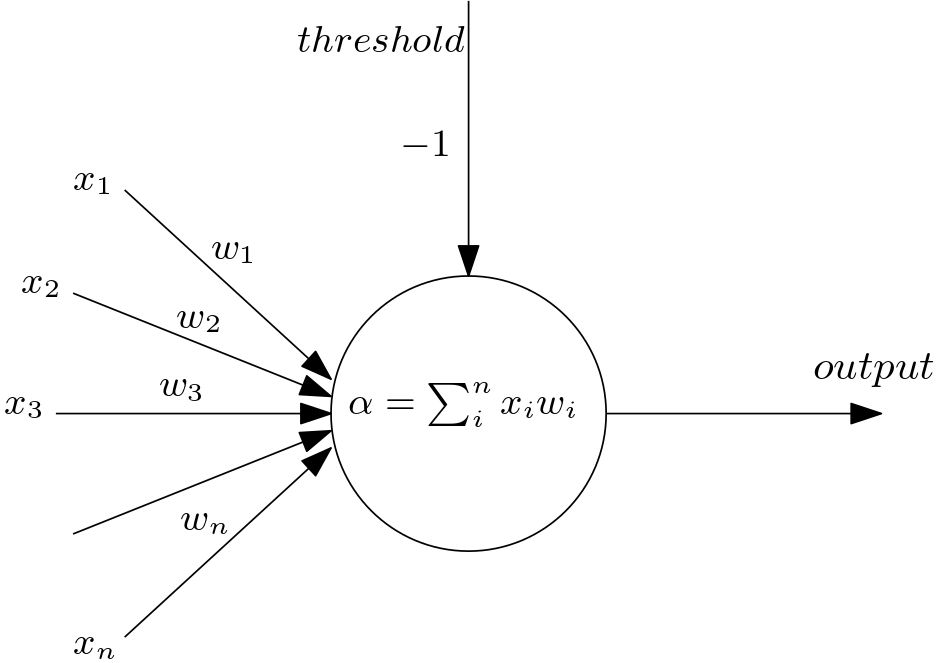
\includegraphics[width=12cm]{perceptron.png}
	\caption{Perceptron \cite{matous}}
	\label{fig:perceptron}
\end{figure}

%=======================================================================================================================
\subsection{Sigmoid Neuron}
Sigmoid neuron, similarly to perceptron, has inputs x and weights. The key difference comes in once we inspect the output value and its calculation.
 Instead of perceptron's binary output 0 or 1, a sigmoid neuron outputs a real number between 0 and 1 using a sigmoid function. \newline
[http://neuralnetworksanddeeplearning.com/chap1.html][8M] \newline
MATH\\
PLOTS\\

As shown in Figure xx and Figure xx, the sigmoid function is a smoothed-out version of the step function.\\
%=======================================================================================================================
\subsection{Activation Function}
An artificial neuron's activation function defines that neuron's output value for given inputs, commonly being ${f: \mathbb{R} \rightarrow \mathbb{R}}$ \cite{leskovec2020mining}. A significant trait of many activation functions is their differentiability, which allows them to be used for \textit{Backpropagation}, ANN algorithm for training weights. The activation function needs to have a derivative that does not saturate by heading towards 0 or explode by heading towards inf \cite{matous}.

For such reasons, the usage of step function or any linear function is unsuitable for ANN.
% Sigmoid Function ==========================================================================================================
\setsecnumdepth{all}
\subsubsection{Sigmoid Function}
The sigmoid function is commonly used in ANN as an alternative to the step function. A popular choice of the sigmoid function is a \textit{logistic sigmoid}. Its output value is in the range of 0 and 1.

\begin{equation}
    {\sigma(\alpha) = \frac{1}{1 + e^{-\alpha}} = \frac{e^x}{1 + e^{x}}}
\end{equation}


% \begin{figure}[h]
%   \centering
%     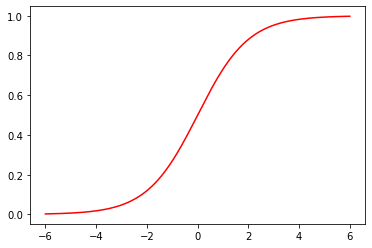
\includegraphics[width=7cm]{sigmoid}
%   \caption{Sigmoid function}
%   \label{fig:sigmoid}
% \end{figure}


One of the reasons for its popularity is the simplicity of its derivative calculation:

\begin{equation}
    {\frac{d}{dx}\sigma(\alpha) = \frac{e^x}{(1 + e^{x})^2} = \sigma(x)(1-\sigma(x))}
\end{equation}


On the other hand, one of its disadvantages is the \textit{vanishing gradient}. A problem where for a given very high or very low input values, there would be almost no change in its prediction. Possibly resulting in training complications or performance issues \cite{7typesactivationfunctions}, \cite{matous}.

% Hyperbolic Tangent ==========================================================================================================

\subsubsection{Hyperbolic Tangent}

Hyperbolic tangent is similar to logistic sigmoid function with a key difference in its output, ranging between -1 and 1.

\begin{equation}
    {tanh(x) = \frac{e^x - e^{-x}}{e^x + e^{-x}}}
\end{equation}


\begin{figure}[h]
    \centering
    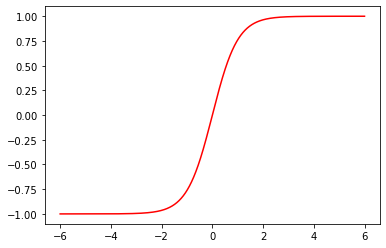
\includegraphics[width=8cm]{tangent}
    \caption{Hyperbolic tangent \cite{matous}}
    \label{fig:hyperbolictangent}
\end{figure}


It shares the sigmoid's simple calculation of its derivative.

\begin{equation}
    {\frac{d}{dx}\tanh(x) = 1 - \frac{(e^x - e^{-x})^2}{(e^x + e^{-x})^2} = 1 -\tanh^2(x)}
\end{equation}

By being only moved and scaled version of the sigmoid function, hyperbolic tangent shares not only sigmoid's advantages but also its disadvantages \cite{leskovec2020mining}, \cite{matous}.

% Rectified Linear Unit ==========================================================================================================

\subsubsection{Rectified Linear Unit}

The output of the Rectified Linear Unit (ReLU) is defined as:

\begin{equation}
    f(x) = max(0,x)
\begin{cases}
    x, & \text{if $x\ \geq\ 0$}\\
    0, & \text{if $x\ <\ 0$}
\end{cases} 
\end{equation} 

\begin{figure}[h]
    \centering
    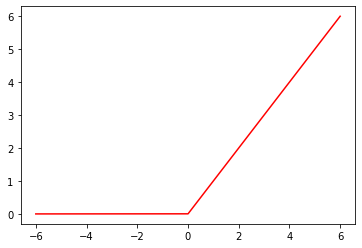
\includegraphics[width=7cm]{relu}
    \caption{Rectified Linear Unit \cite{matous}}
    \label{fig:relu}
\end{figure}


ReLU's popularity is mainly due to its computational efficiency \cite{7typesactivationfunctions}. Its disadvantages appear when inputs approach zero or to a negative number. Causing the so-called dying ReLu problem, where the network is unable to learn. There are many variations of ReLu to this date, e.g., Leaky ReLU, Parametric ReLU, ELU, ...
% Softmax ==========================================================================================================

\subsubsection{Softmax}

Softmax separates itself from all the previously mentioned functions by its ability to handle multiple input values in the form of a vector $\vec{x} = (x_1,x_2,...,x_n)$ and output for each $x_i$ defined as:

\begin{equation}
    {\sigma(x_i) = \frac{e^x_i}{\sum_{j=1}^{n}e^x_j}}
\end{equation}


For output being normalized distribution probability distribution, which ensures $\sum_{i}\sigma(x_i) = 1$ \cite{lipton2015critical}. It is being used as the last activation function of ANN to normalize the network's output into $n$ probability groups.

%=======================================================================================================================
%=======================================================================================================================
\section{Types of Neural Networks}
A
B
C
%=======================================================================================================================\newpage\cleardoublepage
	%========================================================================================================
	\setsecnumdepth{all}
	\chapter{Gesture Recognition}\label{ch:gesture_recognition}
	
Gestures are classified into static gestures and dynamic gestures. Group of static gestures consits of fixed gestures which are not relative to time, where group of dynamic gestures are time varying.

Hand and body gesture recognition had followed a conventional scheme of extracting key features via one or multiple preprocessing sensors and applying machine learning techniques on them.\cite{avola}

The field of gesture recognition gave birth to several image processing devices yielding useful data. One of them being Microsoft Kinect, a device where the main intention was to interpret whole-body movement, making it lacking in required accuracy for hand gesture recognition. 

\section{Leap Motion Controller}
%=======================================================================================================================

Another option would be using a Leap Motion Controller (LMC), developed specifically to track hand movements and extract its features, such as positions of fingers, hand rotation, and others.

LMC consists of two monochromatic IR cameras and three IR LEDs (emitters). 

\begin{figure}[h]
	\centering
    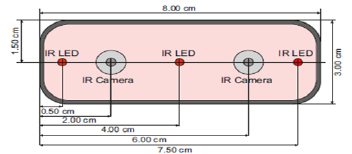
\includegraphics[width=8cm]{lmc_schematic.png}
	\caption{Schematic View of Leap Motion Controller}
	\label{fig:lmcScheme}
\end{figure}



The LMC's current API, Leap Motion Service, yields positions of extracted hand features. All the positional data about the hand and its features are represented in the coordinate system relative to the LMC's center point, positioned at the middle IR LED.\cite{LMCanalysis} The x- and z-axes lie in the camera sensors plane, with the x-axis running along the camera baseline. The y-axis is vertical, with positive values increasing upwards (in contrast to the downward orientation of most computer graphics coordinate systems). The z-axis has positive values increasing toward the user.\cite{tomasMultileap}

\begin{figure}[h]
	\centering
    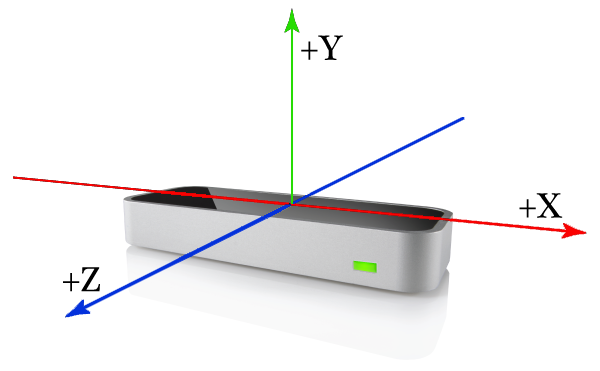
\includegraphics[width=8cm]{leap_axes.png}
	\caption{Leap Motion Controller Axes}
	\label{fig:lmcScheme}
\end{figure}

Unfortunately, Leap Motion Controller has no official library for gesture recognition, limiting developers from utilizing the controller for its key features. Orion, Leap Motion tracking software build for virtual reality, used to have a gesture detector with its 3.0 version, but the detector is absent with the release of more accurate version 4.0.

\section{Methods}
%=======================================================================================================================

Gestures classification should be taken into account when choosing appropriate methods due to their time-varying properties. As previously mentioned, gestures are classified into static and dynamic groups.

\subsection{Static Gesture Recognition}

Common methods for static gesture recognition are Support Vector Machines(SVM), ANN, or pattern techniques.\cite{savaris}.
Mapari and Kharat\cite{mapari} proposed a method to recognize American Sign Language (ASL) by extracting data from LMC and computing 48 features 
(18 positional values, 15 distance values, and 15 angle values) for 4672 collected signs (146 users for 32 signs), eventually feeding them to an ANN using a Multilayer Perceptron (MLP).\cite{katiacnn} Hasan et al.\cite{hasanmlp} proposed a method to recognize six sets of static gestures base on shape analysis using MLP.
Filho et al.\cite{filaml} compared the effectiveness between K-Nearest Neighbors, SVM, and Decision Trees over a dataset of 1200 samples (6 uses for 10 gestures). They normalized positions of the five fingertips and the four angles between adjacent fingers as features to discover that the Decision Tree has performed the best.\cite{katiacnn}

\subsection{Dynamic Gesture Recognition}

\subsection{LSTM}
Many of the proposed methods focus either on static gesture recognition or dynamic gesture recognition, but very few of them are actually utilized for both types at the same time. \newpage\cleardoublepage
	%========================================================================================================
	\setsecnumdepth{all}
	\chapter{MultiLeap}\label{ch:multileap}
	
In 2018, developers from UltraLeap had released an experimental build for Leap Motion tracking software, which provided data from all connected LMCs at once. Despite having this feature, the provided tracking information for the same hand was different from each sensor due to different points of origin. This problem was solved by MultiLeap library created by Tomáš Nováček et al. in \cite{tomasMultileap}, which merges the information from all sensors and returns unified stream of data. The library works with same data structures as Leap Motion's API.

\section{Alignment of the tracking data}

To align tracking data, we must first determine the position of LMCs in order to place them in the virtual world. This can be achieved by computing sensor's positions and rotations in relation to other LMCs \cite{tomasMultileap}.

\subsection{Data sampling}

The MultiLeap library allows a user to sample data using a semi-automatic sampling process. Each sample consists of 20 points from the hand – the points represent the center of each finger joint. 

The sampling is enabled manually, but data are sampled automatically per every Leap Motion frame, approximately 90 times per second. The general idea of automatic sampling is to calibrate sensors using data from already calibrated devices.

First, one sensor is marked as calibrated. The first marked sensor is either the first connected sensor or one selected by the user. Uncalibrated sensors start acquiring samples if the presented hand is in their field of view and at the same time in the field of view of any calibrated sensor. The pair of samples consists of uncalibrated sensor's original data and fused data from all calibrated sensors, to which is the hand visible. Once the sensor collects enough samples, it begins to compute the optimal translation and rotation of the device. The sensor is then marked as calibrated. The process is repeated until all sensors are calibrated \cite{tomasMultileap}.


Hands will then align automatically, but it is up to the user, performing the calibration, to cover enough space of the tracking area. It is best to have diverse samples for more accurate alignment \cite{tomasMultileap}.

Considering the tracking data, where the hand is completely still, it will not have the necessary diversity in its samples. The deviation between collected tracking data is too insignificant. If we were to move the hand across the tracking area, having it rotated in various ways in various positions, the deviation of rotations and positions will be more evident, and the calculation of the alignment more precise \cite{tomasMultileap}.

Another option for calibration is a fully manual setting, allowing a user to set the position and rotation of sensors. Values need to be calculated accurately for the alignment to have any use. The main advantage of this approach is having the possibility of tracking different parts of the tracked space with the sensors, for example, LMCs being back to each other \cite{tomasMultileap}.

The combined approach is also possible. First, making a rough calibration manually and eventually improved by the semi-automatic.

\subsection{Kabsch algorithm}

Kabsch algorithm \cite{kabsch} also known as Procrustes superimposition, was used to determine the rotation of sensors by calculating optimal rotation matrix minimizing the root mean squared deviation between two paired sets of points. The first set of points consists of merged tracking information from calibrated sensors. The second set of points consists of the tracking information from any other sensor. \cite{tomasMultileap}

The goal of the Kabsch algorithm is to compute the optimal translation rotation of P onto Q, where P and Q are sets of pair points that minimize the distance between the two sets. Both P and Q are represented as $N \times 3$ matrix. Each row consists of coordinates of every point \cite{tomasMultileap}.

\begin{equation}
    \begin{pmatrix}
        x_1 & y_1 & z_1\\
        x_2 & y_2 & z_2\\
        \vdots & \vdots & \vdots\\
        x_N & y_N & z_N
    \end{pmatrix}
\end{equation}

Coordinates of the first point are in the first row, the second point in the second row, and the $N$th point in the $N$th row.

The algorithm has two main steps, computing the optimal translation, and computation of the optimal matrix.

The optimal translation can be easily found by being the offset between the averages of two sets of points. As for optimal rotation, we must first calculate the mean center of the points by subtracting the coordinates of the respective centroid from the point coordinates. The centroid $C_P$ for $P$ is computed as follows:

\begin{equation}
    {C_P = {\frac{\sum_{i=1}^{N}P_i}{N}}}
\end{equation}

The mean-center calculation of all points in P:

\begin{equation}
    {P_i = P_i - C_P}
\end{equation}

Then, the $3\times3$ cross-variance matrix between the points must be calculated as follows in matrix notation:

\begin{equation}
    {H = P^T Q}
\end{equation}

At last, we will extract the rotation from the covariance matrix using polar decomposition. The extraction can be done in more iterations, resulting in more accurate rotation calculation but requiring higher computation time in return.

\begin{algorithm}
	\caption{Kabsch algorithm}
	\label{alg:devicePositioning}
	\hspace*{\algorithmicindent} \textbf{Input}: 
	    \begin{itemize}
	        \item \textbf{sensors}: List of N collections of samples for N sensors
	        \item \textbf{iterations}: The number of iterations of the Kabsch algorithm
	    \end{itemize}
	\begin{algorithmic}[1]
		\For {$sensor=2,\ldots,N$}
		    \State optimalTranslation = getAverage(referenceMatrix) - getAverage(sensorMatrix);
			\State covarianceMatrix = transpose(sensorMatrix) - referenceMatrix
			\For {$i=1,\ldots,iterations$}
		    	\State extractRotation(covarianceMatrix)
		    \EndFor
		    \State Translation and rotation of the sensor in the Unity scene
		\EndFor
	\end{algorithmic} 
\end{algorithm}

\section{Data fusion}

If multiple sensors detect the hand, the fusion algorithm is used. In most cases, not all sensors detect the hands properly. One of the yield information provided by MultiLeap library is a \textit{confidence}, a float value ranging from 0.3 to 1, which denotes the confidence level of the tracking data corresponding Leap Motion frame. The purpose of confidence level is to give more weight to tracking data from the sensor, which detects the hand better, making the tracking more accurate even if two out of three sensors would send inaccurate tracking data. The confidence level is of value 0.3 when the palm normal is in a 90\textdegree \xspace and 1 when in 0\textdegree \xspace or 180\textdegree \xspace angle to Y-axis. MultiLeap does not use the confidence of 0 because even with the occlusion of fingers and hand, the tracking data still carries some information about the hand. After few experiments, the value 0.3 was determined to be the most suitable confidence level for minimal tracking data when the palm normal is in 90\textdegree \xspace angle to the Y-axis of the sensor. The mentioned approach resulted in following equation for \textit{confidence} computation:

\begin{equation}
    {confidence = (0.283699 \times angle^2)-(0.891268 \times angle)+1}
\end{equation}

The function transfers the angle, in radians, between the palm normal and the sensor's normal to the corresponding confidence level \cite{tomasMultileap}.

The confidence level is used to give weight to data from the sensor which detects the hand better, making the tracking more precise despite faulty data coming from other sensors.\newpage\cleardoublepage
	%========================================================================================================
	\setsecnumdepth{all}
	\chapter{Implementation}\label{ch:implementation}
	
As briefly mentioned in the Introduction chapter, our goal is to utilize Leap Motion controllers combined with the pre-trained ANN model. In the following chapters, we will explore datasets used for our training and the obstacles that came along with them. Then we will discuss the model training itself and its results. At last, we will deploy the trained model for real-time recognition in a C++ environment.


\section{Dataset Description}

Among many publicly available datasets for gesture recognition are only a few containing necessary skeletal information similar to those yield by Leap Motion controllers. We have selected ASL Dataset and SHREC 2017 Dataset created in conjunction with \cite{avola} and \cite{shrec} respectively, often used as benchmark measurement for trained model accuracy.

\subsection{SHREC 2017 Dataset}

The SHREC dataset contains sequences of 14 dynamic hand gestures. Each gesture was performed between 1 and 10 times by 28 participants in two ways, using one finger and the whole hand. All participants were right-handed. The length of sample gestures varies between 20 to 170 frames, making some samples too short. We solved this by using the padding technique to an acceptable value of $T=100$ \cite{shrec}.

\subsection{ASL Dataset}

ASL Dataset consists of 30 hand gestures, 18 static gestures, and 12 dynamic gestures. Gestures were collected from 20 different people. 13 were used to form the training set, while the remaining 7 formed a test set. Each person performed 30 hand gestures twice, once for each hand, and each gesture is composed of fixed 200 frames as oppose to frame varying SHREC dataset \cite{avola}. 

Unfortunately, after further inspection of the ASL dataset, we have discovered possible mislabeling of features. Specifically, taking a look at internal angles of gesture for number 1, we can see that 1 requires the ring finger to straighten out instead of the index finger. The same can be said about the gesture of number 2, where it appears to have the ring finger and middle finger straight out instead of the index finger and middle finger. It is unclear whether there are other mislabeling among the features. The mislabeling in itself is not an obstacle for training because the features are independent of each other, and the ANN can still learn on them, but the issue will arise in real-time classification, where raw data must be preprocessed identically as the training data. We decided not to use ASL Dataset for our purposes but only to benchmark model architecture.


\subsection{Handicrafted Dataset}

By not using ASL Dataset we have lost a set of static gestures. Also, we want to have the ability to provide the training with our own sets of gestures and not to be bound only to those publicly available. For such purposes, we had created a simple interactive data sampler in the form of a console application.

The sampler saves each sample in .txt format, one line by timestep $T$, frame yield by LMC, each line containing a set of features. Features were selected and computed as previously described in chapter 2.3.3.1. The order of features in a line $x_t$, at time $t$ is as follows.


\begin{equation}
	{x_t = \{\omega_0, ...,\omega_4, \beta_0, ..., \beta_4, u_0,v_0,z_0, ..., u_5,v_5,z_5, \gamma_1, \gamma_2, \gamma_3\}}
\end{equation}



All samples contain the same number of timesteps, specified at the beginning by the user. 

The recording is initiated by key command, but the data collection does not start until the user's hand is in LMC's field of view. Data collection stops once the set of collected frames $\Theta$ matches $T$, or if the hand falls out of LMC's view. Features of missing timesteps are then set as zeroes. The sampling can be subdivided into 3 types:

\begin{enumerate}
	\item \textbf{Single recording} records and saves a single sample. The next recording must be initiated by the user.
    \item \textbf{Open recording} records and saves samples continuously. We recommend using the method only for static gestures. It is best to have full control over recording a dynamic gesture, its beginning, and its end, along with its most significant sequence.
    \item \textbf{Recording significant frames} records and saves a single sample. The next recording must be initiated by the user. The number of collected frames $\Theta^*$ is greater than the required number of timesteps $|\Theta^*| > T$. The last frame is excluded if $|\Theta^*|$ is not even. We will then calculate a \textit{significance} of between $x_t$ and $x_{t+1}$.
    The \textit{significance} of an interval is calculated as euclidean distances of palm positions $P$ between $x_t$ and $x_{t+1}$.

    \begin{equation}
        {s_{(t, t+1)} = d(P_{t}, P_{t+1})}
    \end{equation}

    \begin{equation}
        {S = \{s_{(0, 1)}, ...,s_{(t, t+1)}\}}
    \end{equation}

    Frames are then selected into $\Theta$ by most significant to least significant till $|\Theta| = T$. The following cases must be considered:
    \begin{itemize}
        \item $|\Theta| + 2 \leq T \land x_t$ and $x_{t+1} \notin \Theta$, both frames $x_t$ and $x_{t+1}$ are to be added to $\Theta$.
        \item $|\Theta| + 1 = T \land x_t$ and $x_{t+1} \notin \Theta$, both $x_t$ and $x_{t+1}$ are possible candidates for $\Theta$ but only one can be added due to the size $|\Theta|$ which would reach the limit after addition of one. In order to decide which to pick we will compare the significance $s_{(t-1, t)}$ and $s_{(t+1, t+2)}$, and pick greater of the two.
        
        It is possible that $x_t$ is the first frame of $\Theta^*$, in which case we will pick $x_{t+1}$ to be included in $\Theta$. On the other hand, if $x_{t+1}$ is the last frame of $\Theta^*$, we will pick $x_t$.
        
        \item $x_{t} \notin \Theta \land x_{t+1} \in \Theta$, frame $x_t$ is picked
        \item $x_{t} \in \Theta \land x_{t+1} \notin \Theta$, frame $x_{t+1}$ is picked
    \end{itemize}
    
    The method is recommended for sampling dynamic gestures. We attempt to capture the most important part of a dynamic gesture, its movement. Unfortunately, we are limited to dynamic gestures with whole hand movement. If the sampling is met with more delicate dynamic gestures performed only by fingers, it won't be able to underline the motion.
\end{enumerate}


\section{Model Training}

We selected Python to be our primary language for training the ANN mode along with the web-based interactive development environment Jupyter Notebook. One of the main reasons to pick Python over other available languages was its wide range of libraries and scientific packages supporting machine learning tasks. Most importantly, Keras, a high-level deep learning API integrated with TensorFlow, enabling the user to create and train model structures in very few steps.

SHREC Dataset and ASL Dataset were used to benchmark the model. For the purpose of real-time recognition, we trained the model on our handicrafted dataset consisting of numbers between 1 to 5 and simple dynamic gestures swipe left and right, where each gesture had 150 to 600 samples, 60 frames per sample, recorded in various angles and positions and speeds. 

Each dataset was then split into 80\% for the training set and 20\% for the testing set, where 10\% of the training set was used for validation. Each feature was then normalized via min-max scaler formula:

\begin{equation}
    { x' = \frac{x - Min(X)}{Max(X)-Min(X)}\;\;\; x \in X}
\end{equation}

\subsection{DLSTM architecture}

At first, we followed the proposed architecture of 4 layers stacked LSTM by Avola D., Bernardi M. et al. \cite{avola}. We trained the model using 800 epochs and 0.0001 learning rate, which were proved to be optimal hyperparameters as described in chapter 2.3.3.2.

Benchmarking the model on SHREC Dataset and ASL Dataset resulted in similar accuracies as in \cite{avola}. Our handicrafted dataset had also achieved high results.

Unfortunately, despite achieving high accuracies on all datasets, the model itself did not perform well in a real-time environment. More specifically, the 4 layered LSTM architecture struggled with dynamic gestures. The model did not learn the gesture in relation to the movement but rather on its most occurring position in the recorded sequence, which in the case of swipe right was the palm's final position. The model successfully classified test samples because all gestures swipe right contained some frames where the palm position was on the right. Once we presented the model in a real-time environment with an open palm on the right, without the swipe movement, it classifies such gesture as swipe right, which is an undesired behavior. 

It is unclear whether the model would perform better with more stacked LSTM layers or not, but we concluded that the architecture was not suitable for our purposes. 

\subsection{Two-Layered Bidirectional LSTM architecture}

After an unsuccessful attempt to utilize DLSTM, we turned over to two-layered bidirectional LSTM architecture proposed in \cite{bidirect_dynam}. The proposed architecture was meant and trained on dynamic gestures only, not knowing if it is suitable for static gestures. On the other hand, static gestures can be treated as a special type of dynamic gesture, having one frame stretched out to the desired number of timesteps. Not to mention our dataset was constructed in a way where static gestures have a slight difference in coordinates between $t$ and $t+1$, making it possible to look at the static gesture as a very slow type of dynamic gesture.

Benchmarking the model on SHREC Dataset and ASL Dataset resulted in similar high accuracies as DLSTM architecture. Our handicrafted dataset had also achieved promising results.

The two-layered bidirectional LSTM architecture was successful in learning dynamic gestures base on its characteristic movement. It was also successful in classifying static gestures.

\section{Real time recognition}

Once the model is trained, we save it in .tf format and import it in a C++ environment using Cppflow API created by Sergio Izquierdo. \cite{cppflow}.

\newpage\cleardoublepage
	%========================================================================================================
	\setsecnumdepth{all}
	\chapter{Experiments}\label{ch:experiments}
	
One other goal of the thesis is to evaluate the recognition performance based on a number of connected LMC sensors and test the capabilities of \nameref{ch:multileap} library in the real-time environment using various layouts with a different number of sensors. Results from one connected sensor served as the reference, mostly whether having multiple LMC sensors does improve the recognition of difficult angles. On the other hand, whether MultiLeap \cite{tomasMultileap} perform correct merging for gestures presented in simple default angles.

We used the demo application and trained model as described in section \ref{real_time_recognition}. The model was trained on our original dataset from section \ref{data_sampling}. 

\section{Testing Method}

For each gesture, we performed 1000 classifications. We did not exclude classifications with corrupt sequences, such as when the LMC sensor did not get a correct hand skeletal alignment of the presented hand. We wanted to emulate genuine user interaction with the LMC. Each gesture was held in various positions and angles in a certain span of time until the number of classification was not satisfied. 

Results of multiple LMC sensors are an average of 5 different automatic calibrations. There is currently no telling how well sensors were calibrated. Therefore, we want to avoid generalizing MultiLeap capabilities base on experiments conducted on only one calibration.

Dynamic gestures were not tested, as it is hard to evaluate the percentage of correct classifications in a continuous stream of data. If we test dynamic gestures without any mix-up with static gestures, it will defeat the purpose of testing in a real-time environment. We want to evaluate the performance when a dynamic gesture is performed in the middle of the sequence of static gestures, as to whether the trained model is capable of recognizing the difference between the static gesture of number 5 as oppose to having number 5 moving quickly to one side, doing a swipe. Despite not dedicating any experiments to dynamic gestures, we can still evaluate responsiveness and general correctness when we perform it. We also want to keep track of times when a static gesture gets misclassified for a dynamic gesture, and what is the percentage of valid classification to determine whether the threshold for prediction probability was not set too high.


\subsection{One Leap Motion Sensor}

Experiments for a single connected sensor were performed with LMC's VRVisualizer to understand better how the skeletal structure, which gets classified, looks. It helps us distinguish whether misclassification is caused by our trained model or by LMC's hand joints misalignment.

\begin{figure}[ht]
    \centering
    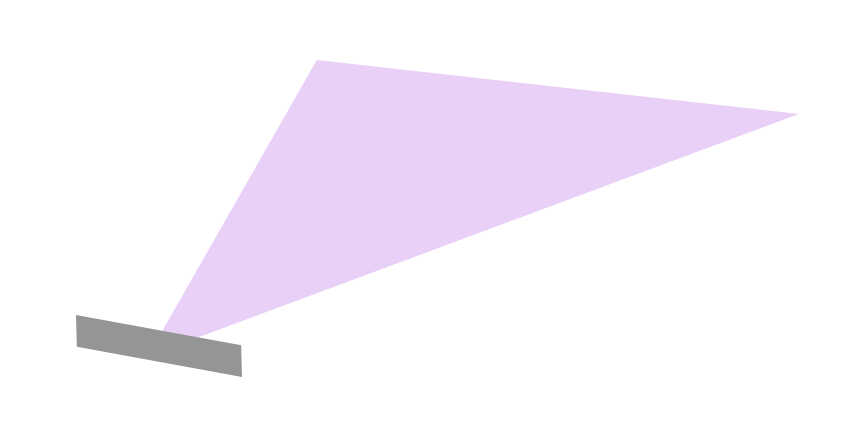
\includegraphics[width=7cm]{setup_1.png}
    \caption{Ilustrative field of view of 1 LMC sensor}
    \label{fig:setup_1}
\end{figure}


The classification was responsive with every presented gesture, including dynamic gestures. Still, the limitation of having only one sensor presents itself when we perform a gesture of \textit{number 1} pointing towards the sensor. The sensor struggles to recognize the pointing finger as being straight, and often time it misclassifies the gesture as a fist, or the prediction does not meet the threshold requirement. It also struggles with the prediction of \textit{number 3} and \textit{number 4}, wherein various angles, the thumb is not recognized by LMC as bent and straighten correctly. Gestures then get confused with \textit{number 2}, and \textit{number 5} respectively. Despite not having  The \textit{pinch} gesture was mostly misclassified due to hand joint misalignment by the LMC sensor. We could be questioning the trained model's performance due to training on a not optimal dataset, but when the hand joint was aligned correctly, the gestures also got classified correctly without any further complications.

The percentage of invalidated gestures was also not too high as most of the discarded predictions were of 0.8 probability and lower. We can assume that our set threshold of 0.9 is not overly strict for the prediction.

\begin{figure}[ht]
    \centering
    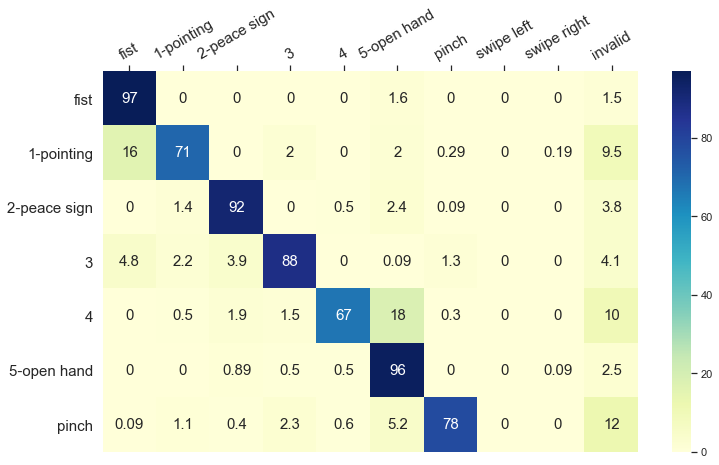
\includegraphics[width=12cm]{one_leap.png}
    \caption{Confusion matrix of prediction by using 1 LMC sensor}
    \label{fig:confuse_1}
\end{figure}


\subsection{Two Leap Motion Sensors}

For two sensors, we explored several layouts with different calibrations. We could not utilize VRVisualizer as we did with one LMC sensor. The MultiLeap library does not have a feature of visualizing the merged hand or any visualization during calibration at the moment. We could not accurately evaluate how the merged hand structure looks like during classification or calibration, thus can be our experiments limited in correction when evaluating the accuracy of multiple LMC sensors. We recommend conducting experiments again once the visualizing feature is implemented.

\subsubsection{Parallel Layout}
\label{parallel_layout}

The parallel layout, with sensors facing each other, could not be tested. LMC sensors expect to receive its emitted IR signals to return from a hand. Instead, the emitted IR signal is received by the other sensor and vice versa. The behavior will confuse LMC recognition making the sensors think there is a hand presented even when it actually is not. Thus we assume this parallel layout is inappropriate to be a part of any setup with multiple LMC sensors.

\begin{figure}[H]
    \centering
    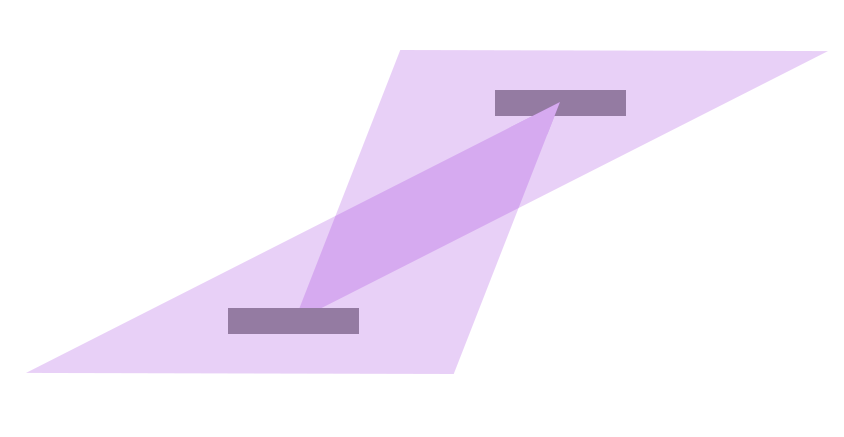
\includegraphics[width=7cm]{setup_2_para.png}
    \caption{Parallel placement layout for 2 LMC sensors}
    \label{fig:setup_2_para}
\end{figure}

\subsubsection{Non-parallel Layout}

Sensors were placed next to each other at a slight angle facing inwards, avoiding sensors to be disturbed by other's emitted IR signals.

\begin{figure}[ht]
    \centering
    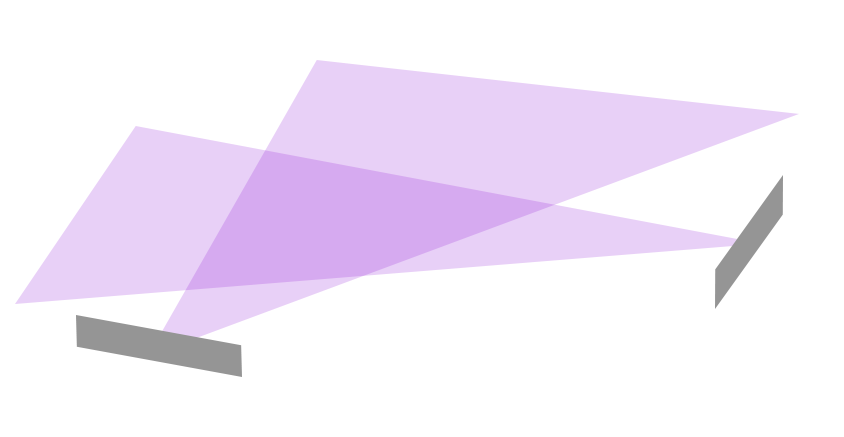
\includegraphics[width=7cm]{setup_2_non.png}
    \caption{Non-parallel placement layout for 2 LMC sensors}
    \label{fig:setup_2_non}
\end{figure}

Using MultiLeap \cite{tomasMultileap} showed improvements in classifying gestures in difficult angles, which it struggled in previous experiments with one connected sensor. The MultiLeap was able to capitalize on the advantage of having multiple fields of view for capturing a presented hand.

Despite improved performance with various angles, the number of invalidated classifications had increased. The average prediction probability for gesture was 0.697, which is most likely caused by misalignment when merging hands. The number of confusion between gestures had also increased. Both could be caused by poor calibration, which there is currently no way to identify the calibration quality in order to avoid this issue. 

\begin{figure}[ht]
    \centering
    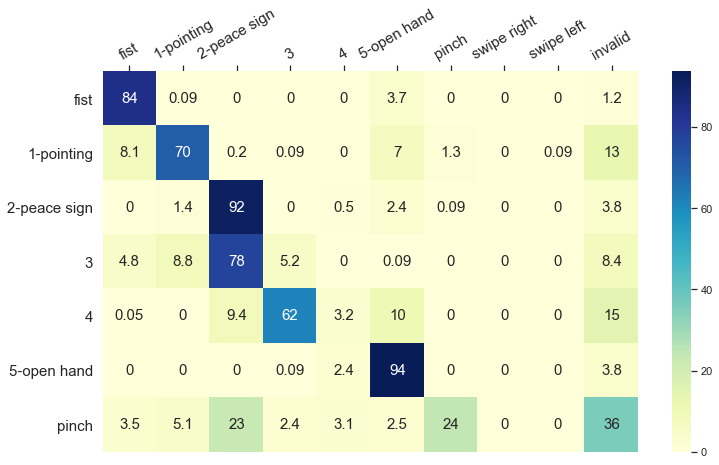
\includegraphics[width=12cm]{two_leap.png}
    \caption{Confusion matrix of prediction by using 2 LMC sensors}
    \label{fig:confuse_2}
\end{figure}

The calibration quality significantly affects the prediction accuracy. More specifically, when we tested \textit{pinch} gesture, the measured average accuracy was mere 24.4\%, but when tested again with a new calibration, the accuracy improved up to 83\%, which is already better than referential results of one connected sensor. The calibration could also have an effect on dynamic gestures. While performing experiments, dynamic gestures were not responsive as they were with only one connected sensor. Often times they were not recognized at all, but their responsiveness varied with different calibrations. 

The MultiLeap's current most notable issue is an incorrect number of reported hands. Our demo application does not make a prediction when there is more than one hand presented. This feature is conflicting with the current bug of MultiLeap, where it frequently returns two hands instead of one, even though only one is present, which from a user's point of view makes the demo application almost unusable for any accurate consecutive recognition. The issue is known, and its fix is currently in development.

\subsection{Three Leap Motion Sensors}

Sensors were carefully placed into a triangular layout so that LMC sensors don't emit IR signals to others, recreating a similar misrecognition issue as in section \ref{parallel_layout}.

\begin{figure}[ht]
    \centering
    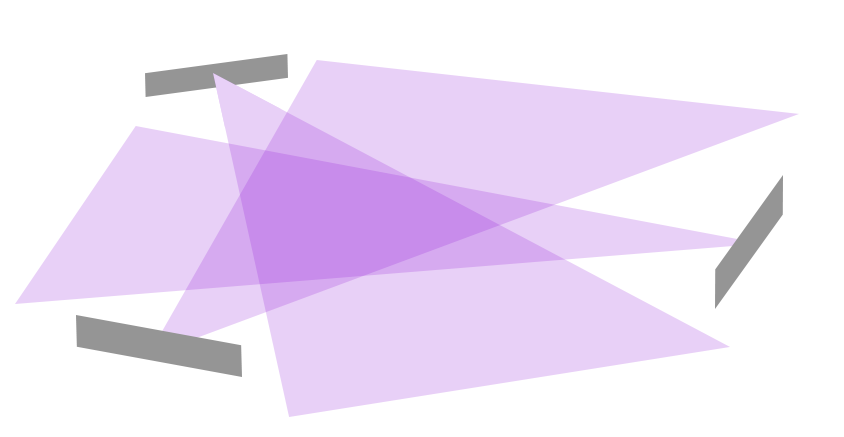
\includegraphics[width=7cm]{setup_3.png}
    \caption{Placement layout for 3 LMC sensors}
    \label{fig:setup_3}
\end{figure}


Using three sensors shares similar behavior as using two sensors. The improvement in recognition of difficult angles was improved upon additional sensors in fewer cases of calibration. Most of the calibrations made did not capitalize properly on the advantage of having multiple sensors. 

The setup suffered similarly, if not at times more, on the side of increased invalidated classification. The average prediction probability for gesture was 0.6841. The issue with the incorrect number of reported hands still persists in a similar frequency as it did with two connected sensors.

\begin{figure}[ht]
    \centering
    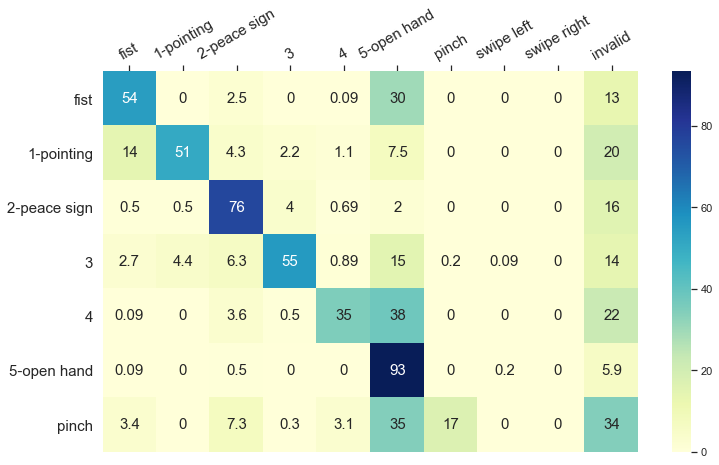
\includegraphics[width=12cm]{three_leap.png}
    \caption{Confusion matrix of prediction by using 3 LMC sensors}
    \label{fig:confuse_3}
\end{figure}

The \textit{pinch} alongside with \textit{number 4} gesture has low accuracy across all 5 different calibrations. They often got confused with the gesture of \textit{number 5}. Dynamic gestures also suffered where the responsiveness seemingly did not change with various calibrations. We can only assume that having more sensors is harder to calibrate and more demanding on calibration quality.



\newpage\cleardoublepage
	%========================================================================================================
	\setsecnumdepth{all}
	\chapter{Conclusion}\label{ch:conclusion}
	The goal of the thesis was to utilize LeapMotion sensors in relation to gesture recognition, creating a pre-trained model and using it to evaluate the capabilities of the MultiLeap library.

We explored publicly available ASL and SHREC datasets, discovered possible feature mislabeling in the ASL dataset, and discussed the dataset's suitability for our purposes. In relation to the discussion, we created a simple way of sampling our dataset with a simplified ability to detect moving sequences while sampling dynamic gestures. We created a dataset consisting of 7 static gestures (fist, 1-pointing, 2-peace sign, 3, 4, 5-open fist, pinch) and 2 dynamic gestures(swipe left, swipe right). Our dataset served the purpose but is not optimal for any benchmark evaluation. Furthermore, the dataset lacks complexity as well as the number of users used for sampling. We suggest expanding the dataset in future works with the engagement of more users, increasing the gesture set as well as its complexity.

ASL dataset, despite its mislabeling, was used for benchmarking and performance evaluation in the testing environment. Our dataset was then used for real-time deployment. Both datasets applied on 4-layered LSTM as well as 2-layered bidirectional LSTM. The 4-LSTM showed promising high results in the testing environment but did not have the desired behavior in real-time deployment due to the inability to learn dynamic gestures, while 2-layered bidirectional LSTM performed well on both fronts. 

We also explored the optimal number of layers and dropout rates for bidirectional LSTMs, resulting in having 2 layers in combination with the 0.6 dropout rate, which is an optimal compromise between accuracy and required training time. As a result, the 2-layered bidirectional LSTM achieved 89.07\% accuracy performing 5-fold cross-validation.

Using the pre-trained model, we created a demo application for debugging and experimental purposes in the form of a simple console application, which supports the connection of multiple Leap Motion sensors. Despite not having an optimal dataset, we achieved to create a responsive classifier for static gestures and dynamic gestures, suitable to be integrated into other applications. However, the application can only classify one hand. Classification of multiple hands would require a new feature structure of the dataset and an improved sliding window solution for real-time recognition. We leave this for future works.

We have conducted several experiments to evaluate the model's performance in the real-time environment and evaluate the performance of the MultiLeap library by using multiple Leap Motion sensors. We explored several setups and the way they can affect Leap Motion detection. We have pointed out issues with the current MultiLeap library alongside its promising results in classifying hand gestures with challenging angles while using multiple sensors. We did not explore all possible setups there are, but it was enough to have a general idea of the current MultiLeap state. We will revisit our setups and explore more in future works with improved MultiLeap.

\newpage\cleardoublepage


\bibliographystyle{iso690}
\bibliography{mybibliographyfile}

\setsecnumdepth{all}
\appendix

\chapter{Acronyms}
% \printglossaries
\begin{description}
	\item[GUI] Graphical user interface
	\item[XML] Extensible markup language
\end{description}


\chapter{Contents of enclosed CD}

%change appropriately

\begin{figure}
	\dirtree{%
		.1 readme.txt\DTcomment{the file with CD contents description}.
		.1 exe\DTcomment{the directory with executables}.
		.1 src\DTcomment{the directory of source codes}.
		.2 wbdcm\DTcomment{implementation sources}.
		.2 thesis\DTcomment{the directory of \LaTeX{} source codes of the thesis}.
		.1 text\DTcomment{the thesis text directory}.
		.2 thesis.pdf\DTcomment{the thesis text in PDF format}.
		.2 thesis.ps\DTcomment{the thesis text in PS format}.
	}
\end{figure}

\end{document}
